\documentclass{article}
\usepackage{graphicx}
\usepackage[margin=1.5cm]{geometry}
\usepackage{amsmath}

\begin{document}

\title{Thursday Reading Assessment: Unit 3, Magnetic Forces and Fields}
\author{Prof. Jordan C. Hanson}

\maketitle

\section{Memory Bank}

\begin{itemize}
\item $\vec{F} = I \vec{L} \times \vec{B}$ ... Lorentz Force on a Current
\item $B = (\mu_0 I)/(2\pi r)$ ... The magnetic field $B$ \textit{caused} by the current $I$ a distance $r$ away.
\item $\mu_0 = 4\pi \times 10^{-7}$ T m A$^{-1}$
\end{itemize}

\begin{figure}[ht]
\centering
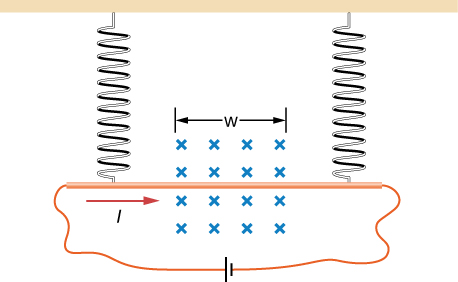
\includegraphics[width=0.35\textwidth]{currentBfieldSpring.jpeg}
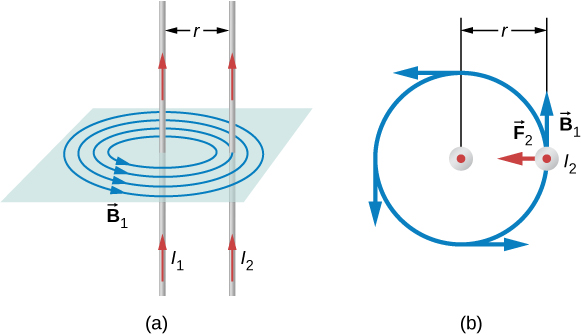
\includegraphics[width=0.35\textwidth]{para.jpeg}
\caption{\label{fig:para} (Left) A current-carrying rod suspended by springs in a B-field.  (Right) Current 1 causes a B-field to exert a Lorentz force on wire 2.  Note that the RHR-2 determines the vector direction of the B-field.}
\end{figure}

\section{Force on a Wire}

\begin{enumerate}
\item Consider Fig. \ref{fig:para} (left). A metal rod of mass m and length L is hung from the ceiling using two springs of spring constant k. A uniform magnetic field of magnitude B pointing perpendicular to the rod and spring exists in a region
of space covering a length w of the copper rod. The ends of the rod are then connected by flexible copper wire across the terminals of a battery. Determine the change in the length $\Delta y$ of the springs when a current I runs through the copper rod, in terms of the other given variables. \\ \vspace{2cm}
\end{enumerate}

\section{Ampere's Law}

\begin{enumerate}
\item Consider Fig. \ref{fig:para}, in which the current $I_1$ \textit{creates} a B-field $\vec{B}$ that encircles $I_1$.  Each wire has a length of 1 meter, is separated by 1 meter from the other, and carries a current of 1 amp in the same direction as the other.  What is the force that $I_1$ exerts on $I_2$?
\end{enumerate}

\end{document}
